% 2005 年全国卷Ⅱ文科第 20 题：直棱锥
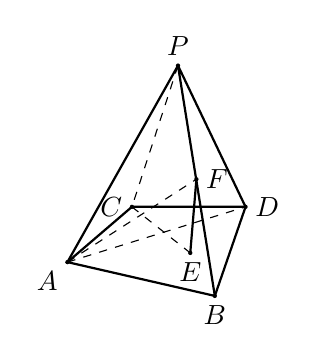
\begin{tikzpicture}[>=stealth,scale=0.78]
  \coordinate (A) at (0,0); \coordinate (B) at (2.4,-0.55);
  \coordinate (C) at (1.05,0.9); \coordinate (D) at (2.9,0.9);
  \coordinate (P) at (1.8,3.2); \coordinate (E) at (2.0,0.15);
  \coordinate (F) at (2.1,1.35);
  \draw[thick] (A)--(B)--(D)--(C)--cycle;
  \draw[thick] (P)--(A) (P)--(B) (P)--(D);
  \draw[dashed] (P)--(C) (A)--(D) (C)--(D);
  \draw[thick] (E)--(F);
  \draw[dashed] (A)--(F) (C)--(E);
  \fill (P) circle (1pt) node[above] {$P$};
  \fill (A) circle (1pt) node[below left] {$A$};
  \fill (B) circle (1pt) node[below] {$B$};
  \fill (C) circle (1pt) node[left] {$C$};
  \fill (D) circle (1pt) node[right] {$D$};
  \fill (E) circle (1pt) node[below] {$E$};
  \fill (F) circle (1pt) node[right] {$F$};
\end{tikzpicture}
